\documentclass[twoside]{book}

% Packages required by doxygen
\usepackage{fixltx2e}
\usepackage{calc}
\usepackage{doxygen}
\usepackage[export]{adjustbox} % also loads graphicx
\usepackage{graphicx}
\usepackage[utf8]{inputenc}
\usepackage{makeidx}
\usepackage{multicol}
\usepackage{multirow}
\PassOptionsToPackage{warn}{textcomp}
\usepackage{textcomp}
\usepackage[nointegrals]{wasysym}
\usepackage[table]{xcolor}

% Font selection
\usepackage[T1]{fontenc}
\usepackage[scaled=.90]{helvet}
\usepackage{courier}
\usepackage{amssymb}
\usepackage{sectsty}
\renewcommand{\familydefault}{\sfdefault}
\allsectionsfont{%
  \fontseries{bc}\selectfont%
  \color{darkgray}%
}
\renewcommand{\DoxyLabelFont}{%
  \fontseries{bc}\selectfont%
  \color{darkgray}%
}
\newcommand{\+}{\discretionary{\mbox{\scriptsize$\hookleftarrow$}}{}{}}

% Page & text layout
\usepackage{geometry}
\geometry{%
  a4paper,%
  top=2.5cm,%
  bottom=2.5cm,%
  left=2.5cm,%
  right=2.5cm%
}
\tolerance=750
\hfuzz=15pt
\hbadness=750
\setlength{\emergencystretch}{15pt}
\setlength{\parindent}{0cm}
\setlength{\parskip}{3ex plus 2ex minus 2ex}
\makeatletter
\renewcommand{\paragraph}{%
  \@startsection{paragraph}{4}{0ex}{-1.0ex}{1.0ex}{%
    \normalfont\normalsize\bfseries\SS@parafont%
  }%
}
\renewcommand{\subparagraph}{%
  \@startsection{subparagraph}{5}{0ex}{-1.0ex}{1.0ex}{%
    \normalfont\normalsize\bfseries\SS@subparafont%
  }%
}
\makeatother

% Headers & footers
\usepackage{fancyhdr}
\pagestyle{fancyplain}
\fancyhead[LE]{\fancyplain{}{\bfseries\thepage}}
\fancyhead[CE]{\fancyplain{}{}}
\fancyhead[RE]{\fancyplain{}{\bfseries\leftmark}}
\fancyhead[LO]{\fancyplain{}{\bfseries\rightmark}}
\fancyhead[CO]{\fancyplain{}{}}
\fancyhead[RO]{\fancyplain{}{\bfseries\thepage}}
\fancyfoot[LE]{\fancyplain{}{}}
\fancyfoot[CE]{\fancyplain{}{}}
\fancyfoot[RE]{\fancyplain{}{\bfseries\scriptsize Generated by Doxygen }}
\fancyfoot[LO]{\fancyplain{}{\bfseries\scriptsize Generated by Doxygen }}
\fancyfoot[CO]{\fancyplain{}{}}
\fancyfoot[RO]{\fancyplain{}{}}
\renewcommand{\footrulewidth}{0.4pt}
\renewcommand{\chaptermark}[1]{%
  \markboth{#1}{}%
}
\renewcommand{\sectionmark}[1]{%
  \markright{\thesection\ #1}%
}

% Indices & bibliography
\usepackage{natbib}
\usepackage[titles]{tocloft}
\setcounter{tocdepth}{3}
\setcounter{secnumdepth}{5}
\makeindex

% Hyperlinks (required, but should be loaded last)
\usepackage{ifpdf}
\ifpdf
  \usepackage[pdftex,pagebackref=true]{hyperref}
\else
  \usepackage[ps2pdf,pagebackref=true]{hyperref}
\fi
\hypersetup{%
  colorlinks=true,%
  linkcolor=blue,%
  citecolor=blue,%
  unicode%
}

% Custom commands
\newcommand{\clearemptydoublepage}{%
  \newpage{\pagestyle{empty}\cleardoublepage}%
}

\usepackage{caption}
\captionsetup{labelsep=space,justification=centering,font={bf},singlelinecheck=off,skip=4pt,position=top}

%===== C O N T E N T S =====

\begin{document}

% Titlepage & ToC
\hypersetup{pageanchor=false,
             bookmarksnumbered=true,
             pdfencoding=unicode
            }
\pagenumbering{alph}
\begin{titlepage}
\vspace*{7cm}
\begin{center}%
{\Large Toposens \\[1ex]\large 0.\+9.\+2 }\\
\vspace*{1cm}
{\large Generated by Doxygen 1.8.13}\\
\end{center}
\end{titlepage}
\clearemptydoublepage
\pagenumbering{roman}
\tableofcontents
\clearemptydoublepage
\pagenumbering{arabic}
\hypersetup{pageanchor=true}

%--- Begin generated contents ---
\chapter{Todo List}
\label{todo}
\Hypertarget{todo}

\begin{DoxyRefList}
\item[\label{todo__todo000001}%
\Hypertarget{todo__todo000001}%
Member \hyperlink{classtoposens__driver_1_1Serial_a43c68993fde1277eff277428d17b47c0}{toposens\+\_\+driver\+:\+:Serial\+:\+:is\+Alive} ()]Since fd is never changed after setup, is there another way to probe? Is this function even useful?  
\item[\label{todo__todo000002}%
\Hypertarget{todo__todo000002}%
Member \hyperlink{classtoposens__driver_1_1Serial_a4837c845aedc74cc1b9a62acb71b0cef}{toposens\+\_\+driver\+:\+:Serial\+:\+:is\+Calibrating} ()]consider if this is even needed  
\item[\label{todo__todo000003}%
\Hypertarget{todo__todo000003}%
Member \hyperlink{classtoposens__driver_1_1Serial_aea7a45dbb1d2edb0b5e60b1cae10584b}{toposens\+\_\+driver\+:\+:Serial\+:\+:send} (char $\ast$bytes)]Use a bit in the header payload to confirm settings update 
\end{DoxyRefList}
\chapter{Class Index}
\section{Class List}
Here are the classes, structs, unions and interfaces with brief descriptions\+:\begin{DoxyCompactList}
\item\contentsline{section}{\hyperlink{classtoposens__driver_1_1Sensor}{toposens\+\_\+driver\+::\+Sensor} }{\pageref{classtoposens__driver_1_1Sensor}}{}
\item\contentsline{section}{\hyperlink{classtoposens__driver_1_1Serial}{toposens\+\_\+driver\+::\+Serial} }{\pageref{classtoposens__driver_1_1Serial}}{}
\end{DoxyCompactList}

\chapter{File Index}
\section{File List}
Here is a list of all documented files with brief descriptions\+:\begin{DoxyCompactList}
\item\contentsline{section}{include/toposens\+\_\+driver/\hyperlink{sensor_8h}{sensor.\+h} \\*Converts raw sensor data to R\+OS friendly structures. Parses a Ts\+Scan from a single input data frame by extracting its header information and the vector of Ts\+Points contained in its payload. Messages are published to topic /ts\+\_\+scans }{\pageref{sensor_8h}}{}
\item\contentsline{section}{include/toposens\+\_\+driver/\hyperlink{serial_8h}{serial.\+h} \\*Provides raw I/O access to TS data stream }{\pageref{serial_8h}}{}
\item\contentsline{section}{src/\hyperlink{serial_8cpp}{serial.\+cpp} \\*Implements serial interface to a TS sensor using native Unix command structures }{\pageref{serial_8cpp}}{}
\end{DoxyCompactList}

\chapter{Class Documentation}
\hypertarget{classtoposens__driver_1_1Sensor}{}\section{toposens\+\_\+driver\+:\+:Sensor Class Reference}
\label{classtoposens__driver_1_1Sensor}\index{toposens\+\_\+driver\+::\+Sensor@{toposens\+\_\+driver\+::\+Sensor}}


{\ttfamily \#include $<$sensor.\+h$>$}

\subsection*{Public Member Functions}
\begin{DoxyCompactItemize}
\item 
\hyperlink{classtoposens__driver_1_1Sensor_ab14040539bf943fcfb95d613ace04f80}{Sensor} (ros\+::\+Node\+Handle nh, ros\+::\+Node\+Handle private\+\_\+nh)
\item 
bool \hyperlink{classtoposens__driver_1_1Sensor_a926de2fe6169b81fb456d2a8d726cebe}{poll} (void)
\item 
void \hyperlink{classtoposens__driver_1_1Sensor_a1a568d4c7946731b20c3f81a3c67a566}{shutdown} (void)
\end{DoxyCompactItemize}
\subsection*{Private Member Functions}
\begin{DoxyCompactItemize}
\item 
void \hyperlink{classtoposens__driver_1_1Sensor_a6ba202a85c681960ce9b31498a942826}{\+\_\+init} (void)
\item 
void \hyperlink{classtoposens__driver_1_1Sensor_a662f061f7fd3181f0ca5527d6f244b6d}{\+\_\+parse} (toposens\+\_\+msgs\+::\+Ts\+Scan \&scan)
\item 
void \hyperlink{classtoposens__driver_1_1Sensor_af20095b07e82801d7827e34622fd604f}{\+\_\+cmd} (char $\ast$out, const char $\ast$key, int val)
\item 
void \hyperlink{classtoposens__driver_1_1Sensor_ab60154cabae56a4ab05230b4fd6222dd}{\+\_\+reconfig} (Ts\+Driver\+Config \&cfg, uint32\+\_\+t level)
\end{DoxyCompactItemize}
\subsection*{Private Attributes}
\begin{DoxyCompactItemize}
\item 
std\+::string \hyperlink{classtoposens__driver_1_1Sensor_ae860cfd52f61f29d80bc086aa722a749}{\+\_\+frame}
\item 
Ts\+Driver\+Config \hyperlink{classtoposens__driver_1_1Sensor_a9542d24036f53f0aebc872554a3802af}{\+\_\+cfg}
\item 
std\+::unique\+\_\+ptr$<$ Cfg $>$ \hyperlink{classtoposens__driver_1_1Sensor_a02f9c1b78374f7958c14260e9fecac70}{\+\_\+srv}
\item 
ros\+::\+Publisher \hyperlink{classtoposens__driver_1_1Sensor_ac18f0d9e465c022a615d526207ff84f3}{\+\_\+pub}
\item 
std\+::unique\+\_\+ptr$<$ \hyperlink{classtoposens__driver_1_1Serial}{Serial} $>$ \hyperlink{classtoposens__driver_1_1Sensor_a202083580774286223129fd84ead26af}{\+\_\+serial}
\item 
std\+::stringstream \hyperlink{classtoposens__driver_1_1Sensor_ad0906c5d74c1da808d26b62d03c54f8d}{\+\_\+data}
\end{DoxyCompactItemize}


\subsection{Detailed Description}
Manages conversion of a single sensor data frame into a Ts\+Scan message. Also provides an interface for configuring sensor performance parameters.

A Ts\+Scan contains timestamped header information followed by a vector of Ts\+Points. A single Ts\+Point has a 3D location (x, y, z) and an associated intenstiy. 

\subsection{Constructor \& Destructor Documentation}
\mbox{\Hypertarget{classtoposens__driver_1_1Sensor_ab14040539bf943fcfb95d613ace04f80}\label{classtoposens__driver_1_1Sensor_ab14040539bf943fcfb95d613ace04f80}} 
\index{toposens\+\_\+driver\+::\+Sensor@{toposens\+\_\+driver\+::\+Sensor}!Sensor@{Sensor}}
\index{Sensor@{Sensor}!toposens\+\_\+driver\+::\+Sensor@{toposens\+\_\+driver\+::\+Sensor}}
\subsubsection{\texorpdfstring{Sensor()}{Sensor()}}
{\footnotesize\ttfamily toposens\+\_\+driver\+::\+Sensor\+::\+Sensor (\begin{DoxyParamCaption}\item[{ros\+::\+Node\+Handle}]{nh,  }\item[{ros\+::\+Node\+Handle}]{private\+\_\+nh }\end{DoxyParamCaption})}

Initiates a serial connection and transmits default settings to sensor. 
\begin{DoxyParams}{Parameters}
{\em nh} & Public nodehandle for pub-\/sub to R\+OS topics. \\
\hline
{\em private\+\_\+nh} & Private nodehandle for retrieving launch parameters.\\
\hline
\end{DoxyParams}
A dynamic reconfigure server is set up to change sensor settings during runtime. 

\subsection{Member Function Documentation}
\mbox{\Hypertarget{classtoposens__driver_1_1Sensor_af20095b07e82801d7827e34622fd604f}\label{classtoposens__driver_1_1Sensor_af20095b07e82801d7827e34622fd604f}} 
\index{toposens\+\_\+driver\+::\+Sensor@{toposens\+\_\+driver\+::\+Sensor}!\+\_\+cmd@{\+\_\+cmd}}
\index{\+\_\+cmd@{\+\_\+cmd}!toposens\+\_\+driver\+::\+Sensor@{toposens\+\_\+driver\+::\+Sensor}}
\subsubsection{\texorpdfstring{\+\_\+cmd()}{\_cmd()}}
{\footnotesize\ttfamily void toposens\+\_\+driver\+::\+Sensor\+::\+\_\+cmd (\begin{DoxyParamCaption}\item[{char $\ast$}]{out,  }\item[{const char $\ast$}]{key,  }\item[{int}]{val }\end{DoxyParamCaption})\hspace{0.3cm}{\ttfamily [private]}}

Constructs a well-\/formed T\+S-\/defined settings command using the passed arguments. 
\begin{DoxyParams}{Parameters}
{\em out} & Pointer to a char buffer where the result will be stored. \\
\hline
{\em key} & Setting name from the k\+Cmd$\ast$ list defined in this class. \\
\hline
{\em val} & Desired value of the setting. Ranges defined in .cfg file. \\
\hline
\end{DoxyParams}
\mbox{\Hypertarget{classtoposens__driver_1_1Sensor_a6ba202a85c681960ce9b31498a942826}\label{classtoposens__driver_1_1Sensor_a6ba202a85c681960ce9b31498a942826}} 
\index{toposens\+\_\+driver\+::\+Sensor@{toposens\+\_\+driver\+::\+Sensor}!\+\_\+init@{\+\_\+init}}
\index{\+\_\+init@{\+\_\+init}!toposens\+\_\+driver\+::\+Sensor@{toposens\+\_\+driver\+::\+Sensor}}
\subsubsection{\texorpdfstring{\+\_\+init()}{\_init()}}
{\footnotesize\ttfamily void toposens\+\_\+driver\+::\+Sensor\+::\+\_\+init (\begin{DoxyParamCaption}\item[{void}]{ }\end{DoxyParamCaption})\hspace{0.3cm}{\ttfamily [private]}}

Transmits settings commands on startup with initial data from the config server.

Only parameters within the root group of cfg Parameter\+Generator broadcast their default values on initialization, so this method only transmits them to the sensor.

Parameters in any sub-\/groups broadcast their value as 0 on startup. It is also possible that sub-\/group params do not broadcast their value on startup, so polling the cfg server returns 0. This is likely a bug with the R\+OS dynamic reconfigure library. \mbox{\Hypertarget{classtoposens__driver_1_1Sensor_a662f061f7fd3181f0ca5527d6f244b6d}\label{classtoposens__driver_1_1Sensor_a662f061f7fd3181f0ca5527d6f244b6d}} 
\index{toposens\+\_\+driver\+::\+Sensor@{toposens\+\_\+driver\+::\+Sensor}!\+\_\+parse@{\+\_\+parse}}
\index{\+\_\+parse@{\+\_\+parse}!toposens\+\_\+driver\+::\+Sensor@{toposens\+\_\+driver\+::\+Sensor}}
\subsubsection{\texorpdfstring{\+\_\+parse()}{\_parse()}}
{\footnotesize\ttfamily void toposens\+\_\+driver\+::\+Sensor\+::\+\_\+parse (\begin{DoxyParamCaption}\item[{toposens\+\_\+msgs\+::\+Ts\+Scan \&}]{scan }\end{DoxyParamCaption})\hspace{0.3cm}{\ttfamily [private]}}

Extracts Ts\+Points from the current data frame and reads them into the referenced Ts\+Scan object. 
\begin{DoxyParams}{Parameters}
{\em scan} & Pointer to a Ts\+Scan for storing parsed data.\\
\hline
\end{DoxyParams}
This O(log n) algorithm only works when the input data frame is exactly in the expected format. Char-\/by-\/char error checks are not implemented so as to increase parsing throughput.

A data frame corresponds to a single scan and has the following format\+: ~\newline
 -\/ Starts with char \textquotesingle{}S\textquotesingle{} ~\newline
 -\/ 6 bytes of frame header info ~\newline
 -\/ Char \textquotesingle{}P\textquotesingle{}, indicates a measured point ~\newline
 -\/ 5 bytes of point header info ~\newline
 -\/ Char \textquotesingle{}X\textquotesingle{}, indicates x-\/coordinate of point ~\newline
 -\/ 5 bytes with measurement of x-\/coordinate ~\newline
 -\/ Char \textquotesingle{}Y\textquotesingle{}, indicates y-\/coordinate of point ~\newline
 -\/ 5 bytes with measurement of y-\/coordinate ~\newline
 -\/ Char \textquotesingle{}Z\textquotesingle{}, indicates z-\/coordinate of point ~\newline
 -\/ 5 bytes with measurement of z-\/coordinate ~\newline
 -\/ Char \textquotesingle{}V\textquotesingle{}, indicates intensity of signal ~\newline
 -\/ 5 bytes with measurement of signal intensity ~\newline
 -\/ ... Additional points in this scan ... ~\newline
 -\/ Ends with char \textquotesingle{}E\textquotesingle{}

In the 6-\/byte long frame header\+: ~\newline
 -\/ First byte is set to 1 when measurements are taken in a noisy ambient environment (hence, likely inaccurate). ~\newline
 -\/ Second byte is currently unused. ~\newline
 -\/ Third byte is set to 1 while sensor calibration is in progress. ~\newline
 -\/ Fourth, fifth and sixth bytes show device address for I2C mode.

The 5-\/byte long pointer header is currently not used. The x-\/, y-\/, z-\/coordinates are calculated in mm relative to the sensor transducer. Signal intensity of the point is mapped to a scale of 0 to 255.

Sample frame\+: S000016\+P0000\+X-\/0415\+Y00010\+Z00257\+V00061\+P0000\+X-\/0235\+Y00019 Z00718\+V00055\+P0000\+X-\/0507\+Y00043\+Z00727\+V00075\+P0000\+X00142\+Y00360\+Z01555\+V00052E ~\newline
 Four points extracted\+: P1(-\/415, 10, 257, 61); P2(-\/235, 19, 718, 55); P3(-\/507, 43, 727, 75); P4(142, 360, 1555, 52) \mbox{\Hypertarget{classtoposens__driver_1_1Sensor_ab60154cabae56a4ab05230b4fd6222dd}\label{classtoposens__driver_1_1Sensor_ab60154cabae56a4ab05230b4fd6222dd}} 
\index{toposens\+\_\+driver\+::\+Sensor@{toposens\+\_\+driver\+::\+Sensor}!\+\_\+reconfig@{\+\_\+reconfig}}
\index{\+\_\+reconfig@{\+\_\+reconfig}!toposens\+\_\+driver\+::\+Sensor@{toposens\+\_\+driver\+::\+Sensor}}
\subsubsection{\texorpdfstring{\+\_\+reconfig()}{\_reconfig()}}
{\footnotesize\ttfamily void toposens\+\_\+driver\+::\+Sensor\+::\+\_\+reconfig (\begin{DoxyParamCaption}\item[{Ts\+Driver\+Config \&}]{cfg,  }\item[{uint32\+\_\+t}]{level }\end{DoxyParamCaption})\hspace{0.3cm}{\ttfamily [private]}}

Callback triggered when a parameter is altered on the dynamic reconfigure server. Determines which setting has changed and transmits the associated (well-\/formed) settings command to the serial stream. 
\begin{DoxyParams}{Parameters}
{\em cfg} & Structure holding updated values of all parameters on server. \\
\hline
{\em level} & Indicates parameter that triggered the callback. \\
\hline
\end{DoxyParams}
\mbox{\Hypertarget{classtoposens__driver_1_1Sensor_a926de2fe6169b81fb456d2a8d726cebe}\label{classtoposens__driver_1_1Sensor_a926de2fe6169b81fb456d2a8d726cebe}} 
\index{toposens\+\_\+driver\+::\+Sensor@{toposens\+\_\+driver\+::\+Sensor}!poll@{poll}}
\index{poll@{poll}!toposens\+\_\+driver\+::\+Sensor@{toposens\+\_\+driver\+::\+Sensor}}
\subsubsection{\texorpdfstring{poll()}{poll()}}
{\footnotesize\ttfamily bool toposens\+\_\+driver\+::\+Sensor\+::poll (\begin{DoxyParamCaption}\item[{void}]{ }\end{DoxyParamCaption})}

Retrieves raw sensor data frames and publishes Ts\+Scans extracted from them. \begin{DoxyReturn}{Returns}
True if scan contains any valid data points. False for an empty scan. 
\end{DoxyReturn}
\mbox{\Hypertarget{classtoposens__driver_1_1Sensor_a1a568d4c7946731b20c3f81a3c67a566}\label{classtoposens__driver_1_1Sensor_a1a568d4c7946731b20c3f81a3c67a566}} 
\index{toposens\+\_\+driver\+::\+Sensor@{toposens\+\_\+driver\+::\+Sensor}!shutdown@{shutdown}}
\index{shutdown@{shutdown}!toposens\+\_\+driver\+::\+Sensor@{toposens\+\_\+driver\+::\+Sensor}}
\subsubsection{\texorpdfstring{shutdown()}{shutdown()}}
{\footnotesize\ttfamily void toposens\+\_\+driver\+::\+Sensor\+::shutdown (\begin{DoxyParamCaption}\item[{void}]{ }\end{DoxyParamCaption})}

Shuts down serial connection to the sensor.

Deletes underlying serial and config server objects managed by class pointers. 

\subsection{Member Data Documentation}
\mbox{\Hypertarget{classtoposens__driver_1_1Sensor_a9542d24036f53f0aebc872554a3802af}\label{classtoposens__driver_1_1Sensor_a9542d24036f53f0aebc872554a3802af}} 
\index{toposens\+\_\+driver\+::\+Sensor@{toposens\+\_\+driver\+::\+Sensor}!\+\_\+cfg@{\+\_\+cfg}}
\index{\+\_\+cfg@{\+\_\+cfg}!toposens\+\_\+driver\+::\+Sensor@{toposens\+\_\+driver\+::\+Sensor}}
\subsubsection{\texorpdfstring{\+\_\+cfg}{\_cfg}}
{\footnotesize\ttfamily Ts\+Driver\+Config toposens\+\_\+driver\+::\+Sensor\+::\+\_\+cfg\hspace{0.3cm}{\ttfamily [private]}}

Maintains current values of all config params. \mbox{\Hypertarget{classtoposens__driver_1_1Sensor_ad0906c5d74c1da808d26b62d03c54f8d}\label{classtoposens__driver_1_1Sensor_ad0906c5d74c1da808d26b62d03c54f8d}} 
\index{toposens\+\_\+driver\+::\+Sensor@{toposens\+\_\+driver\+::\+Sensor}!\+\_\+data@{\+\_\+data}}
\index{\+\_\+data@{\+\_\+data}!toposens\+\_\+driver\+::\+Sensor@{toposens\+\_\+driver\+::\+Sensor}}
\subsubsection{\texorpdfstring{\+\_\+data}{\_data}}
{\footnotesize\ttfamily std\+::stringstream toposens\+\_\+driver\+::\+Sensor\+::\+\_\+data\hspace{0.3cm}{\ttfamily [private]}}

Buffer for storing a raw data frame. \mbox{\Hypertarget{classtoposens__driver_1_1Sensor_ae860cfd52f61f29d80bc086aa722a749}\label{classtoposens__driver_1_1Sensor_ae860cfd52f61f29d80bc086aa722a749}} 
\index{toposens\+\_\+driver\+::\+Sensor@{toposens\+\_\+driver\+::\+Sensor}!\+\_\+frame@{\+\_\+frame}}
\index{\+\_\+frame@{\+\_\+frame}!toposens\+\_\+driver\+::\+Sensor@{toposens\+\_\+driver\+::\+Sensor}}
\subsubsection{\texorpdfstring{\+\_\+frame}{\_frame}}
{\footnotesize\ttfamily std\+::string toposens\+\_\+driver\+::\+Sensor\+::\+\_\+frame\hspace{0.3cm}{\ttfamily [private]}}

Frame ID assigned to Ts\+Scan messages. \mbox{\Hypertarget{classtoposens__driver_1_1Sensor_ac18f0d9e465c022a615d526207ff84f3}\label{classtoposens__driver_1_1Sensor_ac18f0d9e465c022a615d526207ff84f3}} 
\index{toposens\+\_\+driver\+::\+Sensor@{toposens\+\_\+driver\+::\+Sensor}!\+\_\+pub@{\+\_\+pub}}
\index{\+\_\+pub@{\+\_\+pub}!toposens\+\_\+driver\+::\+Sensor@{toposens\+\_\+driver\+::\+Sensor}}
\subsubsection{\texorpdfstring{\+\_\+pub}{\_pub}}
{\footnotesize\ttfamily ros\+::\+Publisher toposens\+\_\+driver\+::\+Sensor\+::\+\_\+pub\hspace{0.3cm}{\ttfamily [private]}}

Topic for publishing Ts\+Scans. \mbox{\Hypertarget{classtoposens__driver_1_1Sensor_a202083580774286223129fd84ead26af}\label{classtoposens__driver_1_1Sensor_a202083580774286223129fd84ead26af}} 
\index{toposens\+\_\+driver\+::\+Sensor@{toposens\+\_\+driver\+::\+Sensor}!\+\_\+serial@{\+\_\+serial}}
\index{\+\_\+serial@{\+\_\+serial}!toposens\+\_\+driver\+::\+Sensor@{toposens\+\_\+driver\+::\+Sensor}}
\subsubsection{\texorpdfstring{\+\_\+serial}{\_serial}}
{\footnotesize\ttfamily std\+::unique\+\_\+ptr$<$\hyperlink{classtoposens__driver_1_1Serial}{Serial}$>$ toposens\+\_\+driver\+::\+Sensor\+::\+\_\+serial\hspace{0.3cm}{\ttfamily [private]}}

Pointer for accessing serial functions. \mbox{\Hypertarget{classtoposens__driver_1_1Sensor_a02f9c1b78374f7958c14260e9fecac70}\label{classtoposens__driver_1_1Sensor_a02f9c1b78374f7958c14260e9fecac70}} 
\index{toposens\+\_\+driver\+::\+Sensor@{toposens\+\_\+driver\+::\+Sensor}!\+\_\+srv@{\+\_\+srv}}
\index{\+\_\+srv@{\+\_\+srv}!toposens\+\_\+driver\+::\+Sensor@{toposens\+\_\+driver\+::\+Sensor}}
\subsubsection{\texorpdfstring{\+\_\+srv}{\_srv}}
{\footnotesize\ttfamily std\+::unique\+\_\+ptr$<$Cfg$>$ toposens\+\_\+driver\+::\+Sensor\+::\+\_\+srv\hspace{0.3cm}{\ttfamily [private]}}

Pointer to config server 

The documentation for this class was generated from the following files\+:\begin{DoxyCompactItemize}
\item 
include/toposens\+\_\+driver/\hyperlink{sensor_8h}{sensor.\+h}\item 
src/sensor.\+cpp\end{DoxyCompactItemize}

\hypertarget{classtoposens__driver_1_1Serial}{}\section{toposens\+\_\+driver\+:\+:Serial Class Reference}
\label{classtoposens__driver_1_1Serial}\index{toposens\+\_\+driver\+::\+Serial@{toposens\+\_\+driver\+::\+Serial}}


{\ttfamily \#include $<$serial.\+h$>$}

\subsection*{Public Member Functions}
\begin{DoxyCompactItemize}
\item 
\hyperlink{classtoposens__driver_1_1Serial_ab66b3b0aba714ac8332d7453833f4294}{Serial} (std\+::string port)
\item 
\hyperlink{classtoposens__driver_1_1Serial_a7970e34fd2b626baa989a7a08e3b2e7f}{$\sim$\+Serial} ()
\item 
bool \hyperlink{classtoposens__driver_1_1Serial_a43c68993fde1277eff277428d17b47c0}{is\+Alive} ()
\item 
bool \hyperlink{classtoposens__driver_1_1Serial_a4837c845aedc74cc1b9a62acb71b0cef}{is\+Calibrating} ()
\item 
void \hyperlink{classtoposens__driver_1_1Serial_a7e1ba7bccecbc978f6e16104ec459e29}{get\+Frame} (std\+::stringstream \&data)
\item 
bool \hyperlink{classtoposens__driver_1_1Serial_aea7a45dbb1d2edb0b5e60b1cae10584b}{send} (char $\ast$bytes)
\end{DoxyCompactItemize}
\subsection*{Private Attributes}
\begin{DoxyCompactItemize}
\item 
int \hyperlink{classtoposens__driver_1_1Serial_a7b3cfddd56ba457aa617737249e197fa}{\+\_\+fd}
\item 
std\+::string \hyperlink{classtoposens__driver_1_1Serial_a7625dc8f63340fc4ea3e076331c5552c}{\+\_\+port}
\item 
const unsigned int \hyperlink{classtoposens__driver_1_1Serial_a383754d17418659020d9f7c221457f5f}{k\+Baud} = B921600
\end{DoxyCompactItemize}


\subsection{Detailed Description}
Low level manager for serial I/O operations. Sets up a U\+A\+RT bridge to access raw data packets from a TS device. Maintains simple read-\/write access at the given baud rate. 

\subsection{Constructor \& Destructor Documentation}
\mbox{\Hypertarget{classtoposens__driver_1_1Serial_ab66b3b0aba714ac8332d7453833f4294}\label{classtoposens__driver_1_1Serial_ab66b3b0aba714ac8332d7453833f4294}} 
\index{toposens\+\_\+driver\+::\+Serial@{toposens\+\_\+driver\+::\+Serial}!Serial@{Serial}}
\index{Serial@{Serial}!toposens\+\_\+driver\+::\+Serial@{toposens\+\_\+driver\+::\+Serial}}
\subsubsection{\texorpdfstring{Serial()}{Serial()}}
{\footnotesize\ttfamily toposens\+\_\+driver\+::\+Serial\+::\+Serial (\begin{DoxyParamCaption}\item[{std\+::string}]{port }\end{DoxyParamCaption})}

Opens a persistent serial connection at the given port. 
\begin{DoxyParams}{Parameters}
{\em port} & Device endpoint usually of the form /dev/tty\+U\+S\+B$\ast$.\\
\hline
\end{DoxyParams}
Various termios struct flags are optimized for a connection that works best with the TS firmware. Any intrinsic flow control or bit processing is disabled.

Connection is a non-\/blocking thread that returns when at least 1 byte is received or 0.\+1s has passed since the last read operation. \mbox{\Hypertarget{classtoposens__driver_1_1Serial_a7970e34fd2b626baa989a7a08e3b2e7f}\label{classtoposens__driver_1_1Serial_a7970e34fd2b626baa989a7a08e3b2e7f}} 
\index{toposens\+\_\+driver\+::\+Serial@{toposens\+\_\+driver\+::\+Serial}!````~Serial@{$\sim$\+Serial}}
\index{````~Serial@{$\sim$\+Serial}!toposens\+\_\+driver\+::\+Serial@{toposens\+\_\+driver\+::\+Serial}}
\subsubsection{\texorpdfstring{$\sim$\+Serial()}{~Serial()}}
{\footnotesize\ttfamily toposens\+\_\+driver\+::\+Serial\+::$\sim$\+Serial (\begin{DoxyParamCaption}\item[{void}]{ }\end{DoxyParamCaption})}

Flushes out bits from the serial pipe and closes its corresponding linux file desciptor. 

\subsection{Member Function Documentation}
\mbox{\Hypertarget{classtoposens__driver_1_1Serial_a7e1ba7bccecbc978f6e16104ec459e29}\label{classtoposens__driver_1_1Serial_a7e1ba7bccecbc978f6e16104ec459e29}} 
\index{toposens\+\_\+driver\+::\+Serial@{toposens\+\_\+driver\+::\+Serial}!get\+Frame@{get\+Frame}}
\index{get\+Frame@{get\+Frame}!toposens\+\_\+driver\+::\+Serial@{toposens\+\_\+driver\+::\+Serial}}
\subsubsection{\texorpdfstring{get\+Frame()}{getFrame()}}
{\footnotesize\ttfamily void toposens\+\_\+driver\+::\+Serial\+::get\+Frame (\begin{DoxyParamCaption}\item[{std\+::stringstream \&}]{data }\end{DoxyParamCaption})}

Extracts a single TS data frame into the given iostream. 
\begin{DoxyParams}{Parameters}
{\em data} & Points to a string stream expecting a sensor frame.\\
\hline
\end{DoxyParams}
Reads incoming bytes to the string stream pointer till the firmware-\/defined frame terminator \textquotesingle{}E\textquotesingle{} is reached. \mbox{\Hypertarget{classtoposens__driver_1_1Serial_a43c68993fde1277eff277428d17b47c0}\label{classtoposens__driver_1_1Serial_a43c68993fde1277eff277428d17b47c0}} 
\index{toposens\+\_\+driver\+::\+Serial@{toposens\+\_\+driver\+::\+Serial}!is\+Alive@{is\+Alive}}
\index{is\+Alive@{is\+Alive}!toposens\+\_\+driver\+::\+Serial@{toposens\+\_\+driver\+::\+Serial}}
\subsubsection{\texorpdfstring{is\+Alive()}{isAlive()}}
{\footnotesize\ttfamily bool toposens\+\_\+driver\+::\+Serial\+::is\+Alive (\begin{DoxyParamCaption}{ }\end{DoxyParamCaption})}

Checks whether or not serial connection is still open. \begin{DoxyReturn}{Returns}
True if connection is open, false otherwise.
\end{DoxyReturn}
Uses the fact that open(3) returns -\/1 if it errors out while opening a serial stream.

\begin{DoxyRefDesc}{Todo}
\item[\hyperlink{todo__todo000001}{Todo}]Since fd is never changed after setup, is there another way to probe? Is this function even useful? \end{DoxyRefDesc}
\mbox{\Hypertarget{classtoposens__driver_1_1Serial_a4837c845aedc74cc1b9a62acb71b0cef}\label{classtoposens__driver_1_1Serial_a4837c845aedc74cc1b9a62acb71b0cef}} 
\index{toposens\+\_\+driver\+::\+Serial@{toposens\+\_\+driver\+::\+Serial}!is\+Calibrating@{is\+Calibrating}}
\index{is\+Calibrating@{is\+Calibrating}!toposens\+\_\+driver\+::\+Serial@{toposens\+\_\+driver\+::\+Serial}}
\subsubsection{\texorpdfstring{is\+Calibrating()}{isCalibrating()}}
{\footnotesize\ttfamily bool toposens\+\_\+driver\+::\+Serial\+::is\+Calibrating (\begin{DoxyParamCaption}{ }\end{DoxyParamCaption})}

Checks the calibration bit of incoming raw data. \begin{DoxyReturn}{Returns}
True if calibration bit is set, false otherwise.
\end{DoxyReturn}
\begin{DoxyRefDesc}{Todo}
\item[\hyperlink{todo__todo000002}{Todo}]consider if this is even needed \end{DoxyRefDesc}
\mbox{\Hypertarget{classtoposens__driver_1_1Serial_aea7a45dbb1d2edb0b5e60b1cae10584b}\label{classtoposens__driver_1_1Serial_aea7a45dbb1d2edb0b5e60b1cae10584b}} 
\index{toposens\+\_\+driver\+::\+Serial@{toposens\+\_\+driver\+::\+Serial}!send@{send}}
\index{send@{send}!toposens\+\_\+driver\+::\+Serial@{toposens\+\_\+driver\+::\+Serial}}
\subsubsection{\texorpdfstring{send()}{send()}}
{\footnotesize\ttfamily bool toposens\+\_\+driver\+::\+Serial\+::send (\begin{DoxyParamCaption}\item[{char $\ast$}]{bytes }\end{DoxyParamCaption})}

Writes the given bytes to the serial stream. Usually used for updating sensor settings during runtime. 
\begin{DoxyParams}{Parameters}
{\em bytes} & Data in a T\+S-\/specific command format (Cxxxxx00000). \\
\hline
\end{DoxyParams}
\begin{DoxyReturn}{Returns}
True if data was transmitted without error. No sensor handshake is received to confirm settings update.
\end{DoxyReturn}
Note that this returns true as long as data is written to the serial stream without error. A success handshake from the sensor confirming the settings update is not currently checked for.

\begin{DoxyRefDesc}{Todo}
\item[\hyperlink{todo__todo000003}{Todo}]Use a bit in the header payload to confirm settings update \end{DoxyRefDesc}


\subsection{Member Data Documentation}
\mbox{\Hypertarget{classtoposens__driver_1_1Serial_a7b3cfddd56ba457aa617737249e197fa}\label{classtoposens__driver_1_1Serial_a7b3cfddd56ba457aa617737249e197fa}} 
\index{toposens\+\_\+driver\+::\+Serial@{toposens\+\_\+driver\+::\+Serial}!\+\_\+fd@{\+\_\+fd}}
\index{\+\_\+fd@{\+\_\+fd}!toposens\+\_\+driver\+::\+Serial@{toposens\+\_\+driver\+::\+Serial}}
\subsubsection{\texorpdfstring{\+\_\+fd}{\_fd}}
{\footnotesize\ttfamily int toposens\+\_\+driver\+::\+Serial\+::\+\_\+fd\hspace{0.3cm}{\ttfamily [private]}}

Linux file descriptor pointing to TS device port. \mbox{\Hypertarget{classtoposens__driver_1_1Serial_a7625dc8f63340fc4ea3e076331c5552c}\label{classtoposens__driver_1_1Serial_a7625dc8f63340fc4ea3e076331c5552c}} 
\index{toposens\+\_\+driver\+::\+Serial@{toposens\+\_\+driver\+::\+Serial}!\+\_\+port@{\+\_\+port}}
\index{\+\_\+port@{\+\_\+port}!toposens\+\_\+driver\+::\+Serial@{toposens\+\_\+driver\+::\+Serial}}
\subsubsection{\texorpdfstring{\+\_\+port}{\_port}}
{\footnotesize\ttfamily std\+::string toposens\+\_\+driver\+::\+Serial\+::\+\_\+port\hspace{0.3cm}{\ttfamily [private]}}

Stored device port for future access. \mbox{\Hypertarget{classtoposens__driver_1_1Serial_a383754d17418659020d9f7c221457f5f}\label{classtoposens__driver_1_1Serial_a383754d17418659020d9f7c221457f5f}} 
\index{toposens\+\_\+driver\+::\+Serial@{toposens\+\_\+driver\+::\+Serial}!k\+Baud@{k\+Baud}}
\index{k\+Baud@{k\+Baud}!toposens\+\_\+driver\+::\+Serial@{toposens\+\_\+driver\+::\+Serial}}
\subsubsection{\texorpdfstring{k\+Baud}{kBaud}}
{\footnotesize\ttfamily const unsigned int toposens\+\_\+driver\+::\+Serial\+::k\+Baud = B921600\hspace{0.3cm}{\ttfamily [private]}}

Baud rate needed for TS device comms. 

The documentation for this class was generated from the following files\+:\begin{DoxyCompactItemize}
\item 
include/toposens\+\_\+driver/\hyperlink{serial_8h}{serial.\+h}\item 
src/\hyperlink{serial_8cpp}{serial.\+cpp}\end{DoxyCompactItemize}

\chapter{File Documentation}
\hypertarget{sensor_8h}{}\section{include/toposens\+\_\+driver/sensor.h File Reference}
\label{sensor_8h}\index{include/toposens\+\_\+driver/sensor.\+h@{include/toposens\+\_\+driver/sensor.\+h}}


Converts raw sensor data to R\+OS friendly structures. Parses a Ts\+Scan from a single input data frame by extracting its header information and the vector of Ts\+Points contained in its payload. Messages are published to topic /ts\+\_\+scans.  


{\ttfamily \#include $<$ros/ros.\+h$>$}\newline
{\ttfamily \#include $<$dynamic\+\_\+reconfigure/server.\+h$>$}\newline
{\ttfamily \#include $<$toposens\+\_\+driver/serial.\+h$>$}\newline
{\ttfamily \#include $<$toposens\+\_\+msgs/\+Ts\+Scan.\+h$>$}\newline
{\ttfamily \#include $<$toposens\+\_\+driver/\+Ts\+Driver\+Config.\+h$>$}\newline
Include dependency graph for sensor.\+h\+:\nopagebreak
\begin{figure}[H]
\begin{center}
\leavevmode
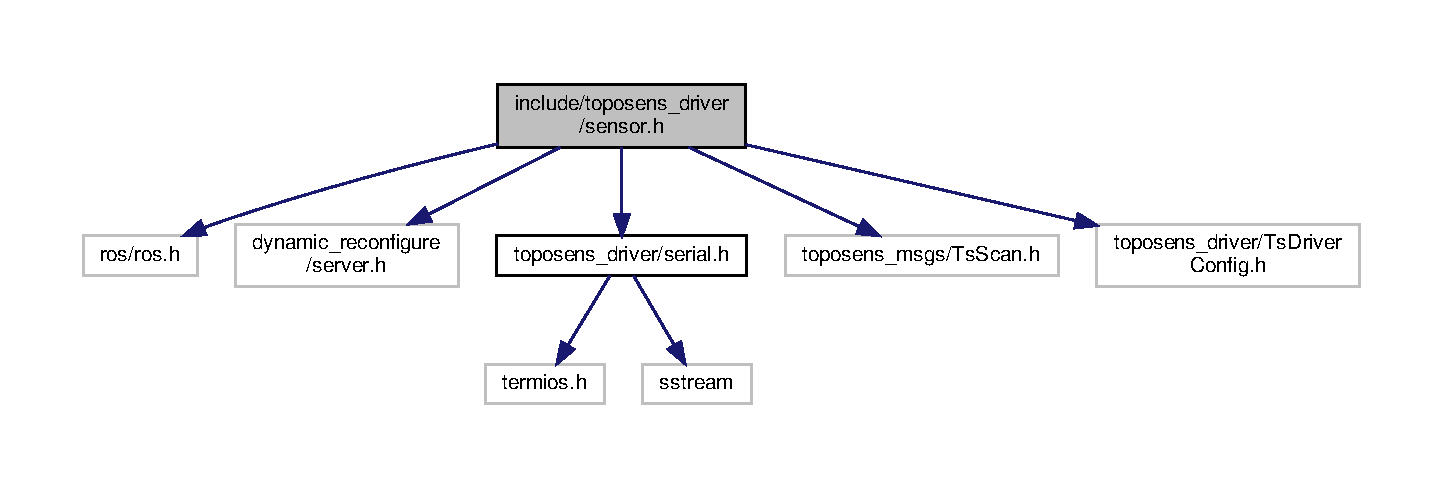
\includegraphics[width=350pt]{sensor_8h__incl}
\end{center}
\end{figure}
\subsection*{Classes}
\begin{DoxyCompactItemize}
\item 
class \hyperlink{classtoposens__driver_1_1Sensor}{toposens\+\_\+driver\+::\+Sensor}
\end{DoxyCompactItemize}
\subsection*{Typedefs}
\begin{DoxyCompactItemize}
\item 
\mbox{\Hypertarget{sensor_8h_ac5fd196ae8358eb0e46089ab8d0d5a0c}\label{sensor_8h_ac5fd196ae8358eb0e46089ab8d0d5a0c}} 
typedef dynamic\+\_\+reconfigure\+::\+Server$<$ Ts\+Driver\+Config $>$ {\bfseries toposens\+\_\+driver\+::\+Cfg}
\end{DoxyCompactItemize}
\subsection*{Variables}
\begin{DoxyCompactItemize}
\item 
\mbox{\Hypertarget{sensor_8h_a349078952764f599a59f4a6c03e85f38}\label{sensor_8h_a349078952764f599a59f4a6c03e85f38}} 
const std\+::string {\bfseries toposens\+\_\+driver\+::k\+Scans\+Topic} = \char`\"{}ts\+\_\+scans\char`\"{}
\item 
\mbox{\Hypertarget{sensor_8h_a7bdf6270301ffcbc9476a88500767a65}\label{sensor_8h_a7bdf6270301ffcbc9476a88500767a65}} 
const int {\bfseries toposens\+\_\+driver\+::k\+Topic\+Queue\+Size} = 100
\item 
\mbox{\Hypertarget{sensor_8h_a92468d435bb77a00e1b3822f9b8d10c3}\label{sensor_8h_a92468d435bb77a00e1b3822f9b8d10c3}} 
const char {\bfseries toposens\+\_\+driver\+::k\+Cmd\+Prefix} = \textquotesingle{}C\textquotesingle{}
\item 
\mbox{\Hypertarget{sensor_8h_a0c1fc858cb001634fe6c6721b7ee21b6}\label{sensor_8h_a0c1fc858cb001634fe6c6721b7ee21b6}} 
const int {\bfseries toposens\+\_\+driver\+::k\+Cmd\+Buffer\+Size} = 100
\item 
\mbox{\Hypertarget{sensor_8h_a26b6704dbfb39d091479c4d424550e44}\label{sensor_8h_a26b6704dbfb39d091479c4d424550e44}} 
const char {\bfseries toposens\+\_\+driver\+::k\+Cmd\+Sig\+Strength} \mbox{[}6\mbox{]} = \char`\"{}n\+Wave\char`\"{}
\item 
\mbox{\Hypertarget{sensor_8h_a019acae90968e7059f034bf3cf3a223b}\label{sensor_8h_a019acae90968e7059f034bf3cf3a223b}} 
const char {\bfseries toposens\+\_\+driver\+::k\+Cmd\+Filter\+Size} \mbox{[}6\mbox{]} = \char`\"{}filtr\char`\"{}
\item 
\mbox{\Hypertarget{sensor_8h_aa7615ca997035c3d7db9d6924bfe78b3}\label{sensor_8h_aa7615ca997035c3d7db9d6924bfe78b3}} 
const char {\bfseries toposens\+\_\+driver\+::k\+Cmd\+Noise\+Thresh} \mbox{[}6\mbox{]} = \char`\"{}d\+Thre\char`\"{}
\item 
\mbox{\Hypertarget{sensor_8h_a22be0a52d0561251dc3134ec57ec1acc}\label{sensor_8h_a22be0a52d0561251dc3134ec57ec1acc}} 
const char {\bfseries toposens\+\_\+driver\+::k\+Cmd\+Voxel\+Limits} \mbox{[}6\mbox{]} = \char`\"{}go\+Lim\char`\"{}
\item 
\mbox{\Hypertarget{sensor_8h_aee2b0e1b9c6da9e9238c9bdc0e67784f}\label{sensor_8h_aee2b0e1b9c6da9e9238c9bdc0e67784f}} 
const char {\bfseries toposens\+\_\+driver\+::k\+Cmd\+Boost\+ShortR} \mbox{[}6\mbox{]} = \char`\"{}slop1\char`\"{}
\item 
\mbox{\Hypertarget{sensor_8h_a03de7c41971f726bd8470a595b44a373}\label{sensor_8h_a03de7c41971f726bd8470a595b44a373}} 
const char {\bfseries toposens\+\_\+driver\+::k\+Cmd\+Boost\+MidR} \mbox{[}6\mbox{]} = \char`\"{}slop2\char`\"{}
\item 
\mbox{\Hypertarget{sensor_8h_aa3d1ab7e7e4f0b7e426e71019e3c7bec}\label{sensor_8h_aa3d1ab7e7e4f0b7e426e71019e3c7bec}} 
const char {\bfseries toposens\+\_\+driver\+::k\+Cmd\+Boost\+LongR} \mbox{[}6\mbox{]} = \char`\"{}slop3\char`\"{}
\end{DoxyCompactItemize}


\subsection{Detailed Description}
Converts raw sensor data to R\+OS friendly structures. Parses a Ts\+Scan from a single input data frame by extracting its header information and the vector of Ts\+Points contained in its payload. Messages are published to topic /ts\+\_\+scans. 

\begin{DoxyAuthor}{Author}
Adi Singh, Sebastian Dengler 
\end{DoxyAuthor}
\begin{DoxyDate}{Date}
January 2019 
\end{DoxyDate}

\hypertarget{serial_8h}{}\section{include/toposens\+\_\+driver/serial.h File Reference}
\label{serial_8h}\index{include/toposens\+\_\+driver/serial.\+h@{include/toposens\+\_\+driver/serial.\+h}}


Provides raw I/O access to TS data stream.  


{\ttfamily \#include $<$termios.\+h$>$}\newline
{\ttfamily \#include $<$sstream$>$}\newline
Include dependency graph for serial.\+h\+:\nopagebreak
\begin{figure}[H]
\begin{center}
\leavevmode
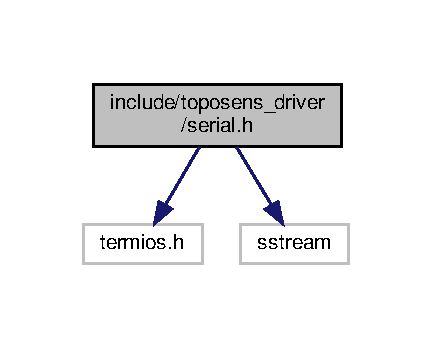
\includegraphics[width=208pt]{serial_8h__incl}
\end{center}
\end{figure}
This graph shows which files directly or indirectly include this file\+:\nopagebreak
\begin{figure}[H]
\begin{center}
\leavevmode
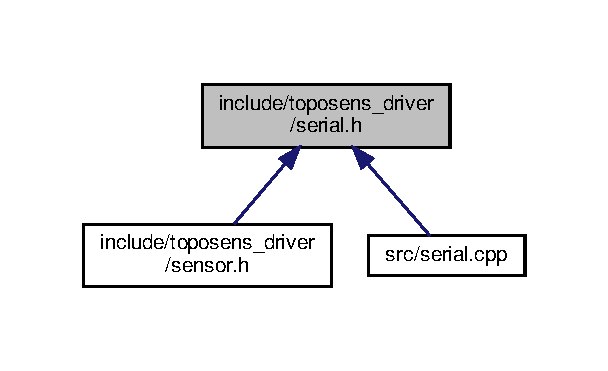
\includegraphics[width=292pt]{serial_8h__dep__incl}
\end{center}
\end{figure}
\subsection*{Classes}
\begin{DoxyCompactItemize}
\item 
class \hyperlink{classtoposens__driver_1_1Serial}{toposens\+\_\+driver\+::\+Serial}
\end{DoxyCompactItemize}


\subsection{Detailed Description}
Provides raw I/O access to TS data stream. 

\begin{DoxyAuthor}{Author}
Adi Singh, Sebastian Dengler 
\end{DoxyAuthor}
\begin{DoxyDate}{Date}
January 2019
\end{DoxyDate}
Methods defined here are independent of R\+OS. 
\hypertarget{serial_8cpp}{}\section{src/serial.cpp File Reference}
\label{serial_8cpp}\index{src/serial.\+cpp@{src/serial.\+cpp}}


Implements serial interface to a TS sensor using native Unix command structures.  


{\ttfamily \#include \char`\"{}toposens\+\_\+driver/serial.\+h\char`\"{}}\newline
{\ttfamily \#include $<$fcntl.\+h$>$}\newline
{\ttfamily \#include $<$ros/console.\+h$>$}\newline
{\ttfamily \#include $<$string.\+h$>$}\newline
Include dependency graph for serial.\+cpp\+:\nopagebreak
\begin{figure}[H]
\begin{center}
\leavevmode
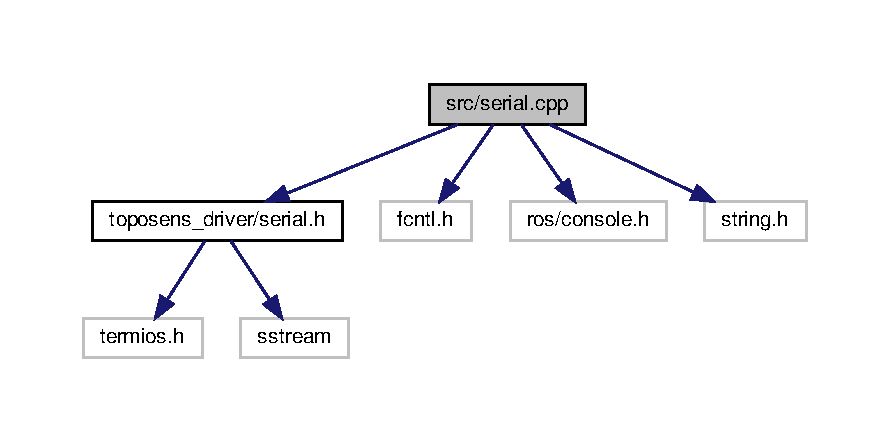
\includegraphics[width=350pt]{serial_8cpp__incl}
\end{center}
\end{figure}


\subsection{Detailed Description}
Implements serial interface to a TS sensor using native Unix command structures. 

\begin{DoxyAuthor}{Author}
Adi Singh, Sebastian Dengler 
\end{DoxyAuthor}
\begin{DoxyDate}{Date}
January 2019
\end{DoxyDate}
Uses ros/console.\+h for outputting R\+O\+S-\/style string messages to terminal. 
%--- End generated contents ---

% Index
\backmatter
\newpage
\phantomsection
\clearemptydoublepage
\addcontentsline{toc}{chapter}{Index}
\printindex

\end{document}
